\documentclass[a4paper]{article}
\usepackage{femape}
\usepackage[lmargin=2cm, rmargin=2cm]{geometry}
\author{Felix Leitl}
\title{Algorithmik kontinuierlicher Systeme}
\begin{document}
\maketitle
\tableofcontents
\newpage
\section{Direkte Verfahren}
Direkte Verfahren Lösen ein Problem nach endlich vielen Schritten. Verwendung: kleine, vollbesetzte Matrizen.
\subsection{LR-Zerlegung}
\subsubsection{Ziel}
\begin{align*}
	A &= LR \\
	\begin{pmatrix}
		a_{11} & \dots & a_{1n} \\
		\vdots & \ddots & \vdots \\
		a_{n1} & \dots & a_{nn}
	\end{pmatrix} &= \begin{pmatrix}
		1 & 0 & \dots & 0 \\
		* & 1 \\
		\vdots &  & \ddots & \vdots\\
		* & & \dots & 1
	\end{pmatrix} \begin{pmatrix}
		* & * & \dots & * \\
		0 & * \\
		\vdots &  & \ddots & \vdots\\
		0 & & \dots & *
	\end{pmatrix}
\end{align*}
\subsubsection{Algorithmus}
\begin{enumerate}
	\item $i$-te Zeile in R übertragen
	\item $i$-te Spalte dividiert durch $a_{ii}$ in L über nehmen. Erstes Element der Spalte gleich 1 setzten 
	\item Mit $i$-ter Zeile die $i$-te Spalte eliminieren 
\end{enumerate}
\subsubsection{Komplexität}
$\BigO(n^3)$
\subsubsection{Anwendung}
\begin{itemize}
	\item $\det(A)=\det(L)\times\det(R)=1\times\det(R)$
	\item Lösen mehrerer GLS:
		\begin{itemize}
			\item $Ly=b$ mit Vorwärtssubstitution $\BigO(n^2)$
			\item $Rx=y$ mit Rückwärtssubstitution $\BigO(n^2)$
		\end{itemize}
\end{itemize}
%TODO: PLR-Zerlegung
\subsubsection{LRP-Zerlegung}
\begin{align*}
	A &= PLR
\end{align*}
\subsection{QR-Zerlegung}
\subsubsection{Ziel}
\begin{align*}
	A = QR
\end{align*}
\subsubsection{Housholder-Spiegelungen}
%TODO: Householder-Spiegelungen
Mit einer Housholder-Spiegelung in eriner Spalte Nullen einfügen (außer Diagonalelement)

$\to$ nach $n-1$ Schritten erhält man die Dreiecksmatrix $R$

\begin{align*}
	R &= H_{n-1}\dots H_2H_1A \\
	Q &= (H_{n-1}\dots H_2H_1)^{-1} = H_1 H_2 \dots H_{n-1}
\end{align*}
\subsubsection{Givens-Rotationen}
Mit einer Givens-Rotation ein Element (unterhalb der Diagonalen) zu Null machen

$\to$ nach $n(n-1)/2$ Schritten erhält man die Dreiecksmatrix $R$

\begin{align*}
	J_{ij}(\varphi)=\begin{pmatrix}
		1 \\
		& \ddots \\
		& & c & &-s \\
		& &  &\ddots \\
		& & s & & c \\
		& & & & & \ddots \\
		& & & & & & 1
	\end{pmatrix}
\end{align*}
Wobei $c_1$ an Position $jj$ ist und $c_2$ an Position $ii$
\begin{align*}
	c &= \cos(\varphi) = \frac{\sigma\cdot a_{jj}}{\sqrt{a^2_{jj}+a^2_{ij}}} \\
	s &= \sin(\varphi)=\frac{-\sigma\cdot a_{ij}}{\sqrt{a^2_{jj}+a^2_{ij}}} \\
	\sigma &= \text{sign}(a_{jj})
\end{align*}
Ergebnis:
\begin{align*}
	R &= J_{m,n^*}\dots J_{2,1}A \\
	Q &= J_{2,1}^T\dots J_{m,n^*}^T \\
	n^* &= \min\{m-1, n\}
\end{align*}
\subsection{Cholesky-Zerlegung}
Wenn $A$ symmetrisch und positiv definit ist kann man A faktorisieren in 
$$
	A=LDL^T
$$
Wobei $L$ das $L$ der LR-Zerlegung ist und $D$ der Diagonalanteil von $R$












\section{Lineare Ausgleichsrechnung}

\section{Matrizen}
\subsection{Orthogonal}
Eine Matrix ist orthogonal, falls eine der Bedingungen erfüllt ist:
\begin{itemize}
	\item $Q^TQ=Id$
	\item $QQ^T=Id$
	\item Spalten oder Zeilen bilden eine Orthonomalbasis
	\item Die Abbildung $Q$ ist winkel- und längentreu
	\item $Q$ erhält das Skalarprdukt: $Qx\circ Qy = x \circ y$
\end{itemize}
\subsection{Skalarprodukt}
$x\circ y=\displaystyle\Sigma_{i=1}^nx_iy_i$
\subsection{Tridiagonalmatrix}
Die inverse einer tridiagonalen Matrix ist in der Regel voll besetzt
\subsection{Normen}
Eigenschaften:
\begin{itemize}
	\item definit: $x\not= 0 \Rarr ||x|| > 0$
	\item homogen: $||\lambda x|| = |\lambda|\cdot||x||$
	\item sub-additiv: $||x+y|| \leq ||x|| + ||y||$
\end{itemize}
\subsubsection{Matrix-Norm bzw. Operator-Norm}
Erfüllt Normeigenschaften und mehr:
\begin{itemize}
	\item $|||Id|||=1$
	\item sub-multiplikativ: $|||AB|||\leq|||A|||\cdot|||B|||$
	\item mit der Vektornorm kompatibel: $||Ax|| \leq |||A|||\cdot||x||$ 
	\item $|||A|||\geq |\lambda|$
\end{itemize}
Beispiele:
\begin{itemize}
	\item Spalten-Summen-Norm: $|||A|||_1$
		$$
			|||A|||_1 = \max_j \{\Sigma_i|a_{ij}|\}
		$$
	\item Zeilen-Summen-Norm: $|||A|||_\infty$
		$$
			|||A|||_\infty = \max_i \{\Sigma_j|a_{ij}|\}
		$$
	\item Spektral-Norm: $|||A|||_2$
		$$
			|||A|||_2 = \sqrt{\lambda\max(A^TA)}
		$$
	\item Frobenius-Norm: $||A||_F$
		$$
			||A||_F = \sqrt{\Sigma_{i=1}^m\Sigma_{j=1}^na_{ij}^2}
		$$
\end{itemize}
\subsubsection{Konditionszahl}
$$
	\kappa(A) = \frac{\max_{x\in\R^n, ||x||=1} ||Ax||}{\min_{x\in\R^n, ||x||=1} ||Ax||}
$$
\subsection{Spektralsatz}
Es sei $A\in\R^{m\times m}$ eine reelle symmetrische Matrix. Dann gibt es eine Orthonomalbasis aus Eigenvektoren bzw. $A=VDV^T$, wobei $D$ die Diagonalmatrix aller EW ist und die Spalten von $V$ die normierten EV sind.
\section{Diskretisierung}

\section{Quantisierung}

\section{Interpolation}

\section{Bezier}
\subsection{Bernstein-Polynom}
$$
	B_i^n(t)=\begin{pmatrix} n \\ i \end{pmatrix}(1-t)^{n-i}t^i
$$
Bildet das Polynom vom Grad $n$

$$
	\begin{pmatrix} n \\ i \end{pmatrix}= \frac{n!}{i!\cdot(n-i)!}
$$
Es gilt:
\begin{itemize}
	\item $0\leq B_i^n(t)\leq1$ für $t\in[0,1]$
	\item $B_i^n(t)$ hat eine $i$-fache Nullstelle in $t=0$
	\item $B_i^n(t)$ hat eine $(n-i)$-fache Nullstelle in $t=1$
	\item $\sum\limits_{i=0}^{n}B_i^n(t)=1 \quad \forall t$
\end{itemize}
\subsection{Formeigenschaften}
\begin{enumerate}
  \item Interpolation der Endpunkte
  \item In den Endpunkten tangetial an das Kontrollpolygon
  \item Bezier-Kurve liegt in der konvexen Hülle der Kontrollpunkte
  \item Affine Invarianz
  \item Variationsreduzierend
\end{enumerate}
\subsection{Auswertung}
\subsubsection{Horner-Bezier}
\begin{align*}
	C(t) &= \sum_{i=0}^n b_i B_i^n (t) \\
	 &= \sum_{i=0}^nb_i \begin{pmatrix} n \\ i \end{pmatrix} (1-t)^{n-i}t^i \\
	 &= (1-t)^n(\tilde b_0 + \tilde b_1 (\frac{t}{1-t})^1 + \dots + \tilde b_n(\frac{t}{1-t})^n) \\
	 &= t^n (\tilde b_0 (\frac{1-t}{t})^n + \dots + \tilde b_{n-1} (\frac{1-t}{t})^{1} + \tilde b_n)
\end{align*}
\subsubsection{de Casteljau}
\begin{center}
	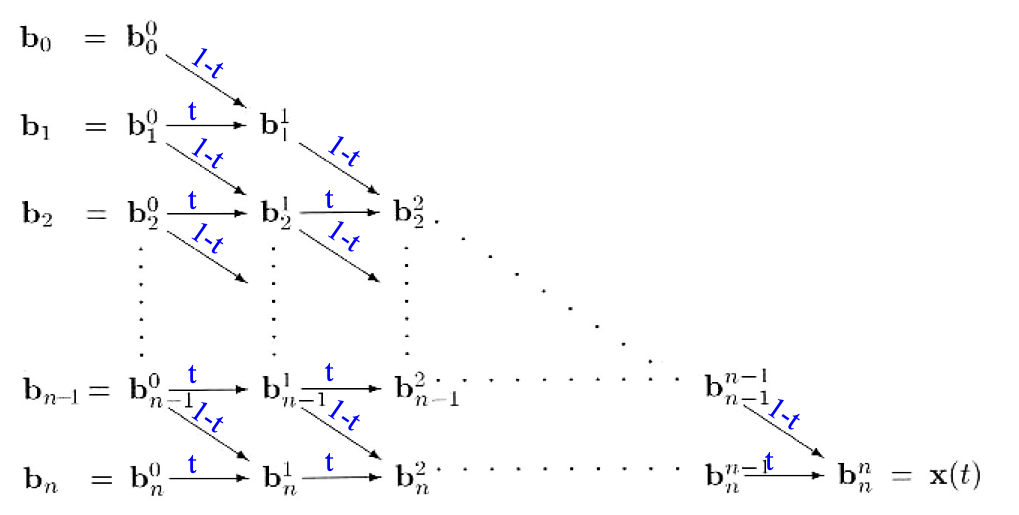
\includegraphics[scale=0.5]{images/de_Casteljau.png}
\end{center}
Durch die Methode der Subdivision mit Hilfe von de Casteljau können Kurven durch kleine Linien sehr effizient dargestellt werden

Durch Rekursion mit Startpunkt in der Mitte konvergiert de Casteljau sehr schnell
\subsection{Glatter Übergang zwischen benachbarten Kurven}
\begin{itemize}
	\item Stetigkeit falls: $b_n = c_0$
	\item Tangenten im Punkt $b_n = c_0$ sind gegeben durch
		\begin{itemize}
			\item $C'(1)=n(b_n-b_n1)$
			\item $B'(0)=n(c_1-c_0)$
		\end{itemize}
	
	Glatt, falls $b_{n-1}, b_n = c_0, c_1$ kollinear sind

\end{itemize}
\subsection{Tensor-Produkt-Bezier-Flächen}
\subsubsection{Allgemein}
$$
	F(s,t) = \sum_{k=0}^m \sum_{i=0}^n b_{ik} B_i^n(s)B_k^m(t)=\sum_{i=0}^n(\sum_{k=0}^m b_{ik} B_k^m(t))B_i^n(t)
$$
Die Kontrollpunkte hängen von $t$ ab
$$
	d_i(t) = \sum_k b_{ik} B_k^m (t)
$$
Kurven mit $s=$const sind Bezier-Kurven in $t$
$$
	F(s,t)=\sum_k c_k(s) B_k^m(t) \text{ mit } c_k(s) = \sum_i b_{ik} B_i^m (s)
$$
Alle Formeigenschaften, außer der Variationsreduktion übertragen sich von den Bezier-Kurven
\subsubsection{Auswertung}
1D Vrsion: Zurrest eindimensional in erste Richtung mit de Casteljau, dann in die andere.

Verallgemeinerung der bilinearen Interpolation: Coons-Patch
\begin{align*}
	P_1 &= C_W(0) = C_S(0) \\
	P_2 &= C_O(0) = C_S(1) \\
	P_3 &= C_N(0) = C_W(1) \\
	P_4 &= C_N(1) = C_O(1)
\end{align*} 
$$
	F_{st}(s,t)=(1-s)(1-t)P_1 + s(1-t)P_2 + (1-s)tP_3 + stP_4
$$
\section{SVD}
$$
	A = U\Sigma V^T
$$
\begin{itemize}
	\item $\Sigma$ ist Diagonalmatrix, $\sigma_{11}\geq\sigma_{22}\geq\dots\geq 0$
	\item $U$ und $V$ sind orthogonal
	\item Die Spalten von $U$ bzw. $V$ sind EV von $AA^T$ bzw. $A^TA$
	\item $\sigma_{kk} = \sqrt{\lambda_k}$ von $A$
	\item $U\in\R^{m\times m}, \Sigma\in\R^{m\times n}, V\in\R^{n\times n}$
\end{itemize}
\subsection{Informationen}
rang$(A)=r$
\subsubsection{Bild}
im$(A)=<u_1, \dots, u_r>$
\subsubsection{Kern}
ker$(A)=<v_{r+1}, \dots, v_n>$
\subsubsection{Norm}
$|||A|||_2=\sigma_{11}$
\subsection{Lösungstheorie}
\begin{itemize}
	\item $n=m$ und $\det(A) \not = 0$: eindeutige Lösung
	\item $n=m$ und $\det(A) = 0$ oder $n\not = m$:
		\begin{itemize}
			\item nur lösbar, falls $b\in$ im$(A)$
			\item alle Lösungen: $x_0 +$ ker$(A)$ wobei $x_0$ eine spezielle Lösung ist  
		\end{itemize}
\end{itemize}
\subsubsection{Pseudo-Inverse}
$$
	A^{\sim1}=V\Sigma^{\sim1}U^T
$$
wobei
$$
	\Sigma^{\sim1}=\begin{pmatrix}
		\frac{1}{\sigma_1} & \dots & 0 & \dots & 0 \\
		\vdots & \ddots & \vdots & & \vdots \\
		0 & \dots & \frac{1}{\sigma_r} & \dots & 0 \\
		\vdots & &  \vdots & 0 & 0 \\
		0 & \dots & 0 & 0 & 0
	\end{pmatrix}
$$
\subsubsection{Lösen}
\begin{itemize}
	\item A hat maximalen Rang $($rank$(A) = \min\{n,m\})$ 
		\begin{itemize}
			\item überbestimmtes System $(n < m)$
		
			$x = A^{\sim1}b$ löst $||Ax-b||=\min$
			\item unterbestimmtes System $(n > m)$
			
			$x = A^{\sim1}b$ löst $Ax=b$ und erfüllst $||x||_2=\min$
		\end{itemize}
	\item rank$(A)<\min\{n,m\}$
		\begin{itemize}
			\item $x = A^{\sim1}b$ minimiert $||Ax-b||_2=\min$ das Residuum und 
			\item ist unter allen diesen Lösungen diejenige mit der kleinsten Norm $||x||_2=\min$
		\end{itemize}
\end{itemize}
\section{Iterative Verfahren}

\end{document}